\documentclass{article}
\usepackage[utf8]{inputenc}
\usepackage{siunitx}
\usepackage{graphics}
\usepackage[american,siunitx]{circuitikz}
\usepackage{amsmath}
\usepackage{svg} 
\usepackage{booktabs}
\usepackage{float}
\usepackage{xparse, xfp}
\usepackage{graphicx} 
\usepackage{steinmetz}
\usepackage{multirow}
\usepackage{pdfpages}
\usepackage{adjustbox}
%\renewcommand{\thesubsection}{\thesection.\alph{subsection}}
\newcommand{\equal}{=}
\newcommand*\circled[1]{\tikz[baseline=(char.base)]{
    \node[shape=circle,draw,inner sep=1pt] (char) {#1};}}

\title{ECE2101L\\Electrical Circuit Analysis II Laboratory\\\,\\Lab 9\\Real, Reactive, Complex Power and Power Factor\\\,\\Report\\}
\author{Choi Tim Antony Yung}
%\author{Choi Tim Antony Yung\\\,\\Willis Nguyen\\Phineas Cozmiuc}

\begin{document}

\clearpage\maketitle
\thispagestyle{empty}
\newpage
\setcounter{page}{1}


\section{Determination of load power using oscilloscope}
\begin{center}
    \begin{adjustbox}{max width=\textwidth}
    \begin{circuitikz}
        \draw 
            (0,0) to[sinusoidal voltage source,v_=$v(t)\equal7cos(2\pi60t)$] (0,-2) node[ground](gnd){}
            (0,0) to[short, i>^=I] ++(0.75,0) to[R=$R\equal\SI{8.2}{\ohm}$] ++(1.5,0) -- ++(0.35,0) node[circ]{} node[above]{\circled{2}} -- ++(0.4,0) coordinate(borderpoint) -- ++(0.5,0) to[R=$R_2\equal\SI{92}{\ohm}$] ++(2.5,0) to[R=$R_3\equal\SI{130}{\ohm}$] ++(2,0) 

            (borderpoint) ++(0.5,0) to[C=\small$C_1\equal\SI{10}{\pico\farad}$] ++(0,-2)
            (borderpoint) ++(3,0) to[L=$L$] ++(0,-2) node[below]{\large{Load}}
            (borderpoint) ++(5,0) to[C=$C_2$] ++(0,-2) -- (gnd)
        ;
        \draw [dashed] (borderpoint) -- ++(0,1) -- ++(6,0) -- ++(0,-3.75) -- ++(-6,0) -- (borderpoint);
    \end{circuitikz}
\end{adjustbox}
\end{center}

\subsection*{Procedure}
The above circuit was simulated with LTspice XVI with the RMS value of source voltage.

\subsection*{Result}
\begin{table}[H]
    \resizebox{\columnwidth}{!}{%
    \begin{tabular}{rcccc}
        \toprule
        Variant & $V_2$ RMS & $I$ RMS & P & Q\\
        & calculated & calculated & calculated & calculated \\
        \midrule
        original & $4.59698\phase{1.66598^{\circ}}$\,V & $46.2263\phase{-20.6450^{\circ}}$\,mA  & 0.196593\,W & 0.0806727\,VAR\\
        \bottomrule    
    \end{tabular} }
    \,\\
    \,\\
    \resizebox{\columnwidth}{!}{%
    \begin{tabular}{rcccccc}
        \toprule
        Variant & $V_2$ RMS & $I$ RMS & P & Q & P & Q \\
        & measured & measured & measured & measured & error & error \\
        \midrule
        original & $4.59698\phase{1.66595^{\circ}}$\,V & $46.2259\phase{-20.6449^{\circ}}$\,mA  & 0.196591\,W & 0.0806715\,VAR & 0.00\% & 0.00\% \\
        $C_2=$\,\SI{1000}{\micro\farad} & $4.61679\phase{1.31314^{\circ}}$\,V & $42.7464\phase{-17.5681^{\circ}}$\,mA  & 0.186732\,W & 0.0638643\,VAR & \multicolumn{2}{c}{\multirow{2}{*}{N/A}} \\
        $L=$\,\SI{0.4}{\henry} & $4.83025\phase{2.21037^{\circ}}$\,V & $27.2304\phase{-56.5461^{\circ}}$\,mA  & 0.068221\,W & 0.1124540\,VAR & \multicolumn{2}{c}{} \\
        \bottomrule    
    \end{tabular} }
    \,\\
    \,\\
    \resizebox{\columnwidth}{!}{%
    \begin{tabular}{rcccl}
        \toprule
        Variant & Load total Z & $|S|$ & PF & \\
        & calculated & calculated & measured &  \\
        \midrule
        original & $107.076\phase{20.6450^{\circ}}$\,$\Omega$ & 0.212501\,VA & 0.925138& lagging\\
        $C_2=$\,\SI{1000}{\micro\farad} & \multicolumn{2}{c}{\multirow{2}{*}{No calculation}} & 0.946191& lagging\\
        $L=$\,\SI{0.4}{\henry}& \multicolumn{2}{c}{} & 0.518677& lagging\\
        \bottomrule    
    \end{tabular} }
\end{table}


\subsection*{Analysis}
From the result we observed that the load power factor have no relation to the magnitude of the load current. The power factor increase with increase of capacitance and decrease with increase of inductance. The angle of load total impedance is roughly the same as the load power angle. Power factor increases with decrease of load power angle and vice versa.


\newpage
\begin{figure}[H]
    \centering
        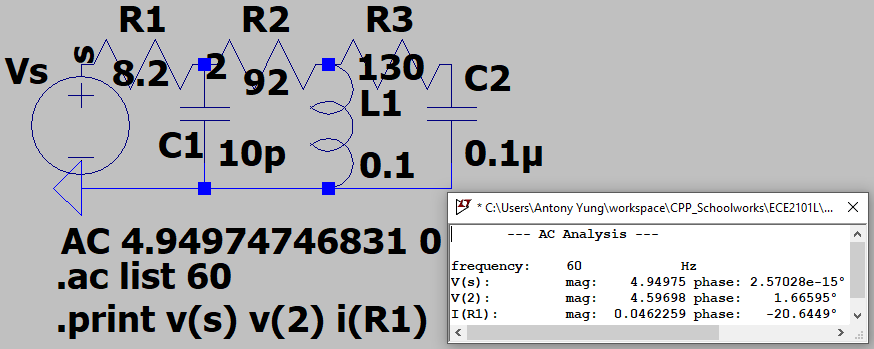
\includegraphics[width=\textwidth]{ECE2101L_Lab09_B1_original.png}
        \caption{Simulation of the original circuit}
\end{figure}

\begin{figure}[H]
    \centering
        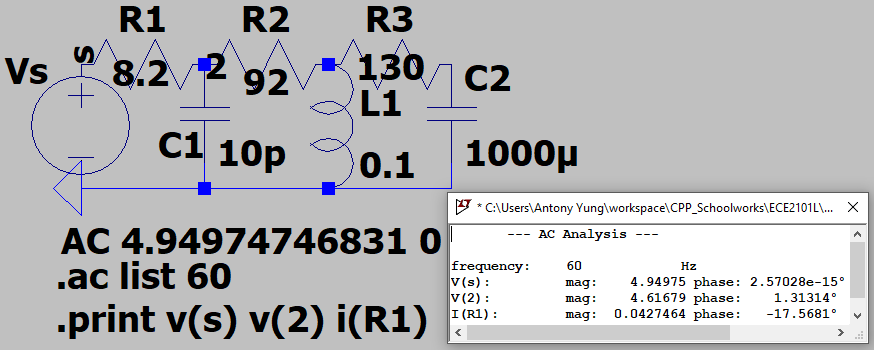
\includegraphics[width=\textwidth]{ECE2101L_Lab09_B1_1000u.png}
        \caption{Simulation of the $C_2=$\,\SI{1000}{\micro\farad} circuit}
\end{figure}

\begin{figure}[H]
    \centering
        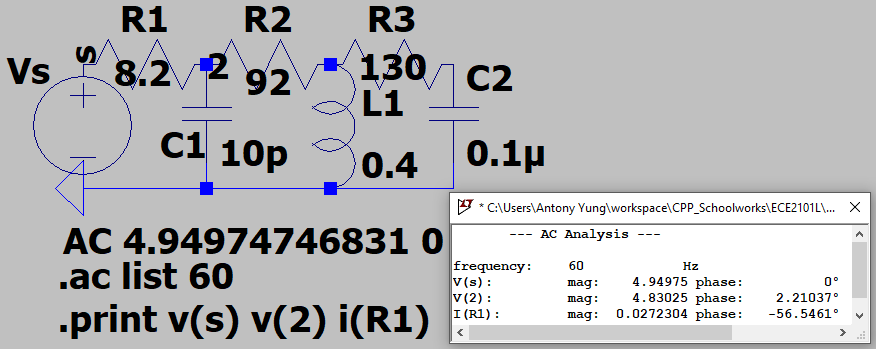
\includegraphics[width=\textwidth]{ECE2101L_Lab09_B1_0.4H.png}
        \caption{Simulation of the $L=$\,\SI{0.4}{\henry} circuit}
\end{figure}

\newpage

\section{Determination of load real power using multimeter}

\subsection*{Procedure}
The original circuit was simulated with LTspice XVI with the RMS value of source voltage and current of $R_2$ and $R_3$.

\begin{figure}[H]
    \centering
        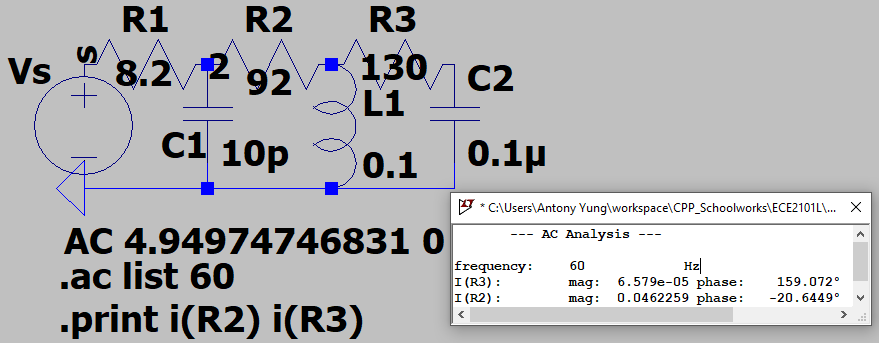
\includegraphics[width=\textwidth]{ECE2101L_Lab09_B2.png}
        \caption{Simulation of the original circuit with measurement of $I_2$ and $I_3$}
\end{figure}

\subsection*{Result}
\begin{table}[H]
    \resizebox{\columnwidth}{!}{%
    \begin{tabular}{rccccc}
        \toprule
        Variant & P from B1 & $I_2$ RMS & $I_3$ RMS & P & P \\
        & measured & measured & measured & measured & error \\
        \midrule
        original & 0.196591\,W & $46.2259\phase{-20.6449^{\circ}}$\,mA  & $65.79\phase{159.072^{\circ}}$\,$\mu$A & 0.196589\,W & 0.00\% \\
        \bottomrule
    \end{tabular} }
\end{table}



\end{document}

